% This is "sig-alternate.tex" V1.9 April 2009
% This file should be compiled with V2.4 of "sig-alternate.cls" April 2009
%
% This example file demonstrates the use of the 'sig-alternate.cls'
% V2.4 LaTeX2e document class file. It is for those submitting
% articles to ACM Conference Proceedings WHO DO NOT WISH TO
% STRICTLY ADHERE TO THE SIGS (PUBS-BOARD-ENDORSED) STYLE.
% The 'sig-alternate.cls' file will produce a similar-looking,
% albeit, 'tighter' paper resulting in, invariably, fewer pages.
%
% ----------------------------------------------------------------------------------------------------------------
% This .tex file (and associated .cls V2.4) produces:
%       1) The Permission Statement
%       2) The Conference (location) Info information
%       3) The Copyright Line with ACM data
%       4) NO page numbers
%
% as against the acm_proc_article-sp.cls file which
% DOES NOT produce 1) thru' 3) above.
%
% Using 'sig-alternate.cls' you have control, however, from within
% the source .tex file, over both the CopyrightYear
% (defaulted to 200X) and the ACM Copyright Data
% (defaulted to X-XXXXX-XX-X/XX/XX).
% e.g.
% \CopyrightYear{2007} will cause 2007 to appear in the copyright line.
% \crdata{0-12345-67-8/90/12} will cause 0-12345-67-8/90/12 to appear in the copyright line.
%
% ---------------------------------------------------------------------------------------------------------------
% This .tex source is an example which *does* use
% the .bib file (from which the .bbl file % is produced).
% REMEMBER HOWEVER: After having produced the .bbl file,
% and prior to final submission, you *NEED* to 'insert'
% your .bbl file into your source .tex file so as to provide
% ONE 'self-contained' source file.
%
% ================= IF YOU HAVE QUESTIONS =======================
% Questions regarding the SIGS styles, SIGS policies and
% procedures, Conferences etc. should be sent to
% Adrienne Griscti (griscti@acm.org)
%
% Technical questions _only_ to
% Gerald Murray (murray@hq.acm.org)
% ===============================================================
%
% For tracking purposes - this is V1.9 - April 2009

\documentclass{sig-alternate}

\usepackage{amssymb}
\setcounter{tocdepth}{3}
\usepackage{graphicx}
\usepackage{xcolor}
\usepackage{subfigure} %[tight,normalsize]
\usepackage{algorithmic}
\usepackage{algorithm}
\usepackage{textcomp}
\usepackage{listings}
\usepackage[T1]{fontenc}
\usepackage{hyperref}
\usepackage{cite} %after hyperref

%\usepackage{url}
%\urldef{\mailsa}\path|{alfred.hofmann, ursula.barth, ingrid.haas, frank.holzwarth,|
%\urldef{\mailsb}\path|anna.kramer, leonie.kunz, christine.reiss, nicole.sator,|
%\urldef{\mailsc}\path|erika.siebert-cole, peter.strasser, lncs}@springer.com|    
%\newcommand{\keywords}[1]{\par\addvspace\baselineskip
%\noindent\keywordname\enspace\ignorespaces#1}

\begin{document}


%
% --- Author Metadata here ---
\conferenceinfo{ESEC/FSE}{'11 SZEGED, HUNGARY}
%\CopyrightYear{2007} % Allows default copyright year (20XX) to be over-ridden - IF NEED BE.
%\crdata{0-12345-67-8/90/01}  % Allows default copyright data (0-89791-88-6/97/05) to be over-ridden - IF NEED BE.
% --- End of Author Metadata ---

%\title{Debugging by {\huge\bf\textit{lastChange}}}
\title{\huge\bf{Querypoint} : Moving Backwards on Wrong Values in the Buggy Execution}

%\subtitle{[Extended Abstract]
%\titlenote{A full version of this paper is available as
%\textit{Author's Guide to Preparing ACM SIG Proceedings Using
%\LaTeX$2_\epsilon$\ and BibTeX} at
%\texttt{www.acm.org/eaddress.htm}}}

%
% You need the command \numberofauthors to handle the 'placement
% and alignment' of the authors beneath the title.
%
% For aesthetic reasons, we recommend 'three authors at a time'
% i.e. three 'name/affiliation blocks' be placed beneath the title.
%
% NOTE: You are NOT restricted in how many 'rows' of
% "name/affiliations" may appear. We just ask that you restrict
% the number of 'columns' to three.
%
% Because of the available 'opening page real-estate'
% we ask you to refrain from putting more than six authors
% (two rows with three columns) beneath the article title.
% More than six makes the first-page appear very cluttered indeed.
%
% Use the \alignauthor commands to handle the names
% and affiliations for an 'aesthetic maximum' of six authors.
% Add names, affiliations, addresses for
% the seventh etc. author(s) as the argument for the
% \additionalauthors command.
% These 'additional authors' will be output/set for you
% without further effort on your part as the last section in
% the body of your article BEFORE References or any Appendices.

\numberofauthors{3} %  in this sample file, there are a *total*
% of EIGHT authors. SIX appear on the 'first-page' (for formatting
% reasons) and the remaining two appear in the \additionalauthors section.
%
\author{
% You can go ahead and credit any number of authors here,
% e.g. one 'row of three' or two rows (consisting of one row of three
% and a second row of one, two or three).
%
% The command \alignauthor (no curly braces needed) should
% precede each author name, affiliation/snail-mail address and
% e-mail address. Additionally, tag each line of
% affiliation/address with \affaddr, and tag the
% e-mail address with \email.
%
% 1st. author
\alignauthor
Salman Mirghasemi\\
       \affaddr{\'Ecole Polytechnique F\'ed\'erale de Lausanne (EPFL), Switzerland}\\
       \email{salman.mirghasemi@epfl.ch}
% 2nd. author
\alignauthor
John J. Barton\\
       \affaddr{IBM Research - Almaden}\\
       \email{bartonjj@us.ibm.com}
% 3rd. author
\alignauthor 
Claude Petitpierre\\
       \affaddr{\'Ecole Polytechnique F\'ed\'erale de Lausanne (EPFL), Switzerland}\\
       \email{claude.petitpierre@epfl.ch}
}       

% There's nothing stopping you putting the seventh, eighth, etc.
% author on the opening page (as the 'third row') but we ask,
% for aesthetic reasons that you place these 'additional authors'
% in the \additional authors block, viz.
% Just remember to make sure that the TOTAL number of authors
% is the number that will appear on the first page PLUS the
% number that will appear in the \additionalauthors section.

\maketitle

\begin{abstract}

\end{abstract}
Developers often seek the origins of wrong values they see in their
debugger. Their search must be backwards in time: the code causing the
wrong value executed before the wrong value appeared. Searching with
breakpoint- or log- based debuggers demands persistence and significant 
experience with the application being debugged.  

\textit{Querypoint}, is a Firefox plugin which enhances the popular 
Firebug JavaScript debugger with a new, practical feature called 
\textit{lastChange}. \textit{lastChange} automatically locates the last point that 
a variable or an object property has been changed. Starting from a 
program halted on a breakpoint, the \textit{lastChange} algorithm 
applies queries to the live program during re-execution, recording 
the call stack and limited program state each time 
the property value changes. When the program halts again on the breakpoint, 
it shows the program state at the last change point. To evaluate the usability and effectivness 
of \textit{Querypoint} we studied four experienced JavaScript developers applying the tool to two test cases.

\category{D.2.5}{Testing and Debugging}{Debugging aids}
\category{D.2.6}{Programming Environments}{Integrated environments}


\terms
{Algorithms, Human Factors, Languages}

\keywords
{Debugging, Locating Defects, Querypoint, LastChange, Breakpoint,
 Watchpoint, Logging}

\section{Introduction}

According to  \cite{LaToza}, developers spend about fifty percent of
their time debugging. To fix a bug, developers typically reproduce 
and monitor the buggy execution several times to understand the 
program's unexpected behavior. Trial-and-error, guess-work, and 
analyzing complicated data make debugging difficult and time-consuming. 
Enhanced debugging operations save  
time, reduce development costs and improve software quality.

A common strategy for locating defects starts from bug symptoms and
works backwards, moving from a point in the program execution where a
value appears to be incorrect back to the point where that value was
set.  Two conventional approaches, breakpoint-based and
log-based debugging, require tedious steps of
selecting data to be collected, collecting the data, then analyzing
the results. 

%In breakpoint debugging, developers select data to be collected by
%searching through source files and setting breakpoints. To determine
%where a value was set incorrectly, a developer must set
%breakpoints at all possible points where the value changes. At
%every breakpoint, the developer must determine if the location is in
%fact related to the questionable value change then study the complex
%debugger user interface and memorize values or manually collect
%data. As the number of breakpoint hits increases, the process of
%checking the program state, collecting data and resuming the execution
%becomes cumbersome.

%In log-based debugging, developers select data to be collected by
%inserting statements for all points of possible change.  While in
%breakpoint-based debugging, the whole program state is available to
%developer, in log-based debugging, developer has to decide what data
%should be collected when inserts the log statement. It is very common
%that the developer has to repeat this step several times due to
%insufficient collected data, or to wait a long time because too much
%data is recorded. Once adequate data is collected, it still
%requires analyzing and understanding. Developers usually end up in
%dealing with long log files and analyzing huge amounts of collected data. 
%Neither approach effectively assists the developer in finding origins to a wrong
%value.

Locating the origin of wrong values becomes even harder when developers 
deal with weakly-typed dynamic languages such as JavaScript. First, due to weakly-typed
nature of these languages the search space that the developer should consider is considerably 
larger than traditional languages such as Java and C{\small\#}. Second, dynamic features make 
program full static analysis almost impossible.

\textit{Querypoint}, is a Firefox plugin which enhances the popular 
Firebug JavaScript debugger with a new, practical feature called 
\textit{lastChange}\cite{Mirghasemi2011}. \textit{lastChange}, locates the origin of a wrong
value by queries on the running program. This feature enables interactive 
dynamic data dependency navigation without requiring a full trace, unlike 
other dynamic slice navigation interfaces. The technique builds on existing 
breakpoint debugger technology  and it does not require a special environment to
create identical, instruction by instruction, re-executions. \textit{Querypoint} 
also provides mechanism for automated bug reproduction, and a novel user interface which
summarizes investigated execution points and collected results.


%Morover, it implements interactive 
% dynamic data dependency navigation for JavaScript, which poses a unique 
% challenge with respect to its dynamic nature. 


%Imagine that a program execution 
%is paused on a breakpoint and the developer is
%suspicious about the value of a variable or an object property. The
%developer selects \textit{lastChange} on the value. The debugger
%replays the buggy execution and collects data when the data field changes. 
%Once the execution reaches the same place (i.e., the same
%breakpoint hit), it pauses the execution, analyzes the collected data
%and shows the location of the last change to the developer. The
%developer can also examine the program state at the located point of
%execution, and continue debugging by more \textit{lastChange} queries
%from that point. 


\section{Related Work}
\label{sec:relatedWork}
%whyline, firecrystal
Most tools developed to enhance developers' navigation on the buggy execution can 
be classifed in two main groups: replay-based and logging-based. Replay-based 
approaches capture limited data during execution and replay the buggy execution 
to reach past points. In contrast, logging-based approaches collect enough data during
execution to relieve developer from re-execution, then query the data to 
inform the developer.

Among replay-based debuggers we can name bdb \cite{Boothe} and
reverse watchpoint \cite{Maruyama}. Both tools rely on deterministic
executions and employ a step counter to locate the requested point from the
beginning of execution. These tools incur two to four times runtime overhead.

Among logging-based debuggers are \textit{omniscient} debuggers (e.g.,
ODB\cite{Lewis}, TOD \cite{Pothier}, Unstuck\cite{Hofer} and WhyLine\cite{Ko}) and
time-travelling debuggers (e.g., Nirvana \cite{Bhansali}). Logging-based debuggers 
suffer from different issues. First, the recording
step is time expensive (20-120 times) and it should be repeated in case of changes in
program. Second, the execution log cannot fully replace the live
execution. There are other aspects of execution (e.g., program user
interface, file system, database tables, etc.) which are also
important in debugging and are not available to the developer in 
logging-based debuggers. Third, querying collected data (e.g., to restore
the program state at a certain point) may not be efficient enough for
debugging realistic programs. 

\textit{Querypoint} resembles the operational model of replay-based debuggers
and the query approach of logging-based debuggers. Contrary to
other replay-based debuggers, which require exactly the same
re-executions (deterministic executions), \textit{Querypoint} only requires \textit{bug 
reproducibility}, meaning a test case is available which reproduces the bug and a 
way to halt execution reliably after the reproduction. Contrary to logging-based
debuggers \textit{Querypoint} selectively collects data which significantly reduces
runtime overhead incured by logging.

%A recent work by Lienhard et al.\cite{Lienhard} suggests virtual
%machine level support for keeping the history of events. It replaces every
%object reference with an alias object which keeps the history of
%changes to the object reference. Although this approach incurs less runtime overhead (7 times) in
%comparison to omniscient debuggers, it adds memory
%overhead. 

% Origin tracking of \texttt{undefined} and \texttt{null} values employing \textit{value piggybacking} technique proposed by
%Bond et al. \cite{Bond}. This approach has two main limitations comparing to \textit{lastChange}.
%First, it is limited to \texttt{undefined} and \texttt{null} values. Second, it does not return the last change
%of a \texttt{null} variable but the first place that the \texttt{null} value is originated.


\section{Querypoint}
\label{sec:introExample}

We illustrate the \textit{Querypoint} functionality by a simple
example. The example demonstrates a buggy JavaScript code in a HTML
page (Figure~\ref{fig:js-code}). The page contains a button (line 40)
showing the value of \texttt{myObject.myProperty}.  When the user
clicks on the button, the \texttt{onClick} function (line 13) is
called. This function increases the value of
\texttt{myObject.myProperty} by one (line 15) and calls
\texttt{updateButton} function which updates the button's text to the new
value (line 22).  Once the page is loaded for the first time, the
button shows \texttt{1} as the initial value of
\texttt{myObject.myProperty}.  In practice when the user clicks on the
button, \texttt{0} appears instead of \texttt{2}: there is a bug.

%Two other functions are called in \texttt{onClick()}, \texttt{foo()}
%and \texttt{bar()}. As developers we often encounter function calls
%which seem peripheral to our current concern; they may have been added
%by another developer, or we may have forgotten their exact properties
%or those properties may have changed, and so on. The difference
%between what we expect these functions to do, e.g. nothing
%interesting, and what they do in practice may cause bugs.


\begin{figure}[htp]

%\includegraphics[width=.5\textwidth]{
%\begin{verbatim}
\lstset{basicstyle=\scriptsize}
\lstset{emph={myProperty},emphstyle=\textit}
%\lstset{backgroundcolor=\color{yellow}}
\lstdefinelanguage{myLang}
{morekeywords={html, script, button, if, function, var}}

\begin{lstlisting}[frame=single, language=myLang] %, framerule=0pt]

1 <html>
...
5   <script type="text/javascript">
6    myObject = {myProperty : 1};
7    myCondition = {value : 1};
...
13   function onClick(){
14     foo();
15     myObject.myProperty++;
16     bar();
17     ...
18     updateButton();
19   }
20   function updateButton(){
21     var myParagraph =
          document.getElementById("myButton");
22     myButton.innerHTML = myObject.myProperty;
23   }   
24   function foo(){
25  	 myCondition.value = oldValue;
26   }  
27   function bar(){ 
28     if (!myCondition.value)
29         myObject.myProperty = 0;
30   }
31  </script> 
...
40  <button id="myButton" onclick="onClick()">
41  	1 
42  </button>
43 </html>
\end{lstlisting}
%\end{verbatim}
\caption{A Web page containing JavaScript code. Some lines not related to our paper have been elided.}
\label{fig:js-code}
\end{figure}

By browsing through the code,% or other means\cite{Barton},
 the developer determines that the value displayed on the 
button is set at line 22. Since the displayed value is incorrect we know 
the bug occurred before we hit this line.
To start debugging, the developer sets a breakpoint
on line 22. Once the button is clicked, the execution is paused at line
22. Figure~\ref{fig:example1} shows the Firebug debugger while the
execution is paused. Firebug has several panels (e.g., HTML, CSS,
Script, DOM, etc.) that each demonstrate one aspect of the Web page.
The Script panel contains the list of all loaded source
files and regular debugging facilities such as setting breakpoints and
stepping. To the right of the script panel, the Watch panel shows the program state
where the developer can examine object and variable values. In our case, the
\texttt{myObject.myProperty} value at the paused point is \texttt{0}. We expected this value to be \texttt{2}.



\begin{figure*}[htp]

\subfigure[A screen shot of the Firebug debugger while running the example code from Fig.~\ref{fig:js-code}. The Script
  panel is selected; it gives access to
  all loaded source files and allows breakpoints to be set on lines. In this
  figure, the execution is paused at line 22 by a regular
  breakpoint. The Watch panel on the right shows the program state at
  the paused
  point. Developer can query \textit{lastChange} on \texttt{myObject.myProperty} by right-clicking on the value of \texttt{myProperty}. ]{\label{fig:example1}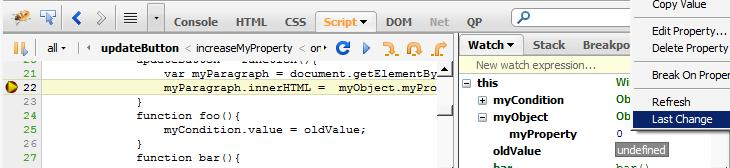
\includegraphics[width=1.0\textwidth, %height=.17\textheight
  ]{1-bp22.jpg}}


\subfigure[The result of \textit{lastChange} query for
  \texttt{myObject.myProperty}. The left panel, QP, shows the source
  code at the point of \textit{lastChange}; The right panel,
  TraceData, shows the collected data at the
  point.]{\label{fig:example3}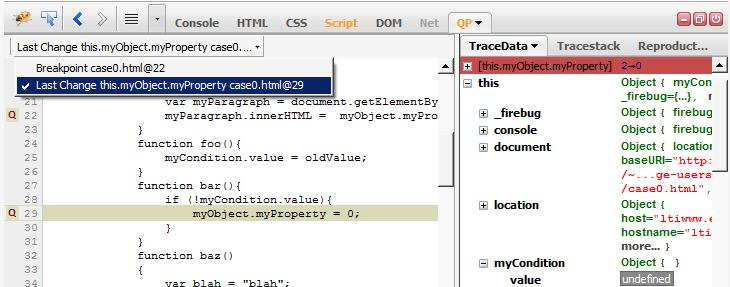
\includegraphics[width=1.0\textwidth,% height=.21\textheight
  ]{3-lastChange.jpg}}

\subfigure[The result of \textit{lastChange} query for
  \texttt{myCondition.value}. To evaluate an expression (e.g., oldValue) at this point, developer can %TODO should we remove it?
  enter the expression in the watch box and after re-execution the result is available.
  The opened list on the top of the left panel shows the visited execution points. Clicking on each point in
  the list shows the corresponding code and
  data.]{\label{fig:example4}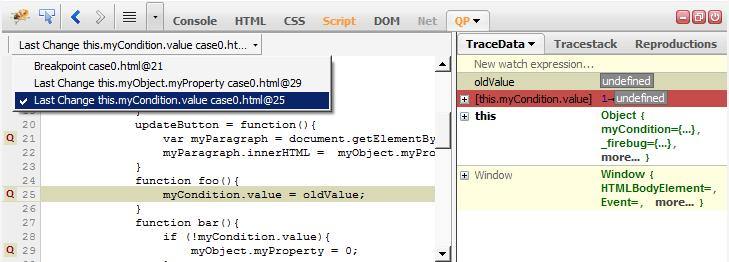
\includegraphics[width=1.0\textwidth%,height=.25\textheight
    ]{4-lastChange2.jpg}}

\caption{The stages of locating the defect using \textit{lastChange} feature.}
\label{fig:lastChange}
\end{figure*}


To apply backward search strategy for locating defects, the developer
first needs to know the origin of the wrong value. To achieve this
goal using breakpoints, the developer should search code to find all possible places that
\texttt{myObject. myProperty} might get a new value and set breakpoint at these locations. However, an
object and property can be accessed and changed through different
names and methods. There is no simple way to identify these aliases or
even their total number.  The developer can make a good guess and set
breakpoints on lines where the property seems to be changed. Then they
re-execute the program and examine the state looking for values that
may lead to the incorrect value observed at line 22. All this work
must be repeated if a new alias is discovered or if some
information related to the buggy result was missed while stopped on
one of the breakpoints.

In contrast, we have added a high-level function in the debugger,
\textit{lastChange}, which provides the answer without tedious manual
effort from the developer. By right clicking on
\texttt{myObject.myProperty} in the Watch panel, the developer can run
\textit{lastChange} command (Figure~\ref{fig:example1}). The debugger
re-executes the program and halts again at the breakpoint on line 22.
However, it shows a new panel, called QP, centered on the source at line 29
(Figure~\ref{fig:example3}), the point of \textit{lastChange}.  To
the right, the TraceData panel shows values of properties of the
program state when it passed through line 29.  These two panels
resemble the Script and Watch panels, but they show data collected by
the debugger at one execution point which is now past: these are
\textit{traces} or \textit{logs} of information collected during the re-execution.

Looking at line 29, it seems that something is wrong with
\texttt{myCondition.value} which causes line 29 execution. The
developer examines \texttt{myCondition.value} and it is
\texttt{undefined}. The next step is to know when this property got
this value. To do so, the developer runs the \textit{lastChange} command
on \texttt{myCondition.value} at this point. The debugger re-executes the
program and breaks again on line 22, analyzes its queries and shows the developer line 25-the
place \texttt{oldValue} is assigned to
\texttt{myCondition.value}. If the developer asks for \textit{lastChange} on \texttt{oldValue}, 
the debugger can notify the developer that this variable is never assigned a value.
 Now it is clear that the bug occurs because \texttt{oldValue} is
\texttt{undefined} once the execution reaches line 25 (Figure~\ref{fig:example4}).


The developer has examined three points of execution. The first point  was the breakpoint set by the developer. 
We call this special breakpoint the \textit{reproduction point}.
The second and third points preceded the reproduction point in execution sequence.
All three points-the history
of the search for the defect-are available through the debugger's
interface. On the top of the left panel in Figure~\ref{fig:example4}
there is an opened list which shows all three examined points. Moreover, the source lines related to these
points are marked with red \textbf{Q} icons.
%The
%first one is the breakpoint on line 22, the second one is the point
%which is when \texttt{myObject.myProperty} changed before
%reaching the breakpoint and finally the last one is the point of
%execution in which \texttt{myCondition.value} gets the
%\texttt{undefined} value. 

%Notice that in our example, \textit{lastChange} combines some aspects
%of breakpoint and of log-based debugging. Like breakpoint debugging,
%the developer re-executes a live runtime without changing the source
%and without a special execution environment beyond the debugger. The
%state of the program memory and the call stack are available at each
%lastChange point. Like log-based debugging, the program state and the
%call stack are recorded during program execution. We can't halt the
%program at \textit{lastChange} because we don't know which point is the last
%one until we return to the original breakpoint. 
%In section 5 we discuss cases where it is possible to pause at lines of \textit{lastChange}.

\textit{Querypoint} needs a test case to reproduce the
execution and conditions to correctly recognize the reproduction point. 
Although both elements can be directly provided by developer, \textit{Querypoint}
is also able to automatically create them from the first execution. 

To replay execution, \textit{Querypoint} keeps track of breakpoint hits and single steps. For example, 
if the developer queries \textit{lastChange} at the third hit of breakpoint \textit{b}, in
re-execution, the third hit is recognized as the reproduction point. \textit{Querypoint} supports two mechanism
for automatic re-execution: callstack-reproduction and record-replay. In callstack reproduction the function from
the earliest frame of the call stack is called with the same parameters. The record-replay execution uses two phases. In the record phase, it 
stores the initial page url and the events and parameters corresponding to user actions. In the replay phase, it opens
the same url and simulates events as if they were user actions. 


In addition to the data collected at every change event for identifying the \textit{lastChange}
result, \textit{Querypoint} partially stores values in program state. There is a trade-off between the amount of data collected at every change event and the number of re-executions. If the developer asks for some values which have not been stored, \textit{Querypoint} re-executes and collects the requested data. 


\section{User Study}
We supplied four experienced Javascript developers with \textit{Querypoint} in an 
extended Firebug debugger\footnote[1]{http://ltiwww.epfl.ch/\texttildelow mirghase/lastchange-userstudy}. Following a tutorial and a practice case, we observed as they 
applied both conventional breakpoint and \textit{lastChange} on two small programs we provided. The first program, Shapes, calculates the area and perimeter values for a list of shapes. The bug happens when one of the calculated numbers is zero. The second program, Moving Circle, randomly scales and moves a circle in the page. The bug happens once the circle becomes invisible after an exception occurs. This case represent a reproducible non-deterministic execution. The developers were asked to locate the defects that caused these bugs. All four developers successfully applied \textit{lastChange} to the test programs and understood how it could help debugging. To find the defect location with breakpoints, all four users took more steps\footnote[2]{A step is a button push, either single stepping the debugger or running a \textit{lastChange query}} and more time (Figure~\ref{fig:userstudy}).    

%another searched the text, a third set a lot of breakpoints to understand the control flow. 
%Based on our own experience we expect these strategies represent the kinds of approaches 
%developers have available. These operations are time consuming and tedious. In contrast, all four users 
%found the defect location with just two \textit{lastChange} operations.

% Based on our measurements,
%this makes \textit{lastChange} about three times faster than breakpoints for the navigation from 
%the reproduction point to the defect
%We recognize that these programs were designed to highlight lastChange and many kinds of debugging 
%issues have been hidden by the design of our tests. Nevertheless our results show that, when a defect 
%relates to incorrect values and a developer recognizes this, then the operational 
%mechanics of lastChange lead to the defect much more quickly than breakpoints.


\begin{figure}[htp]
\centering 
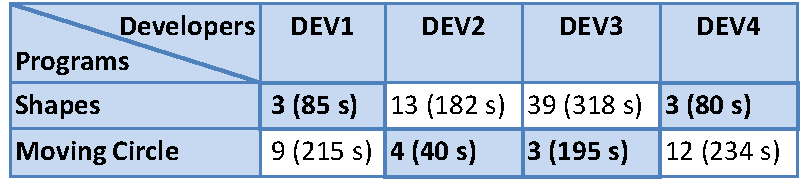
\includegraphics[width=.48\textwidth]{10-userstudy.pdf}
\caption{The number of steps (and time in seconds) required before locating a defect, for each test subject and test program. 
Cells with a white background report values with conventional debugging; Cells with a colored background use \textit{lastChange}.}

\label{fig:userstudy}
\end{figure}


\section{Conclusion and Future Work}
\textit{Querypoint} provides critical information for debugging Jav- aScript programs: 
the location and state at the point where a questionable value was assigned. It only requires 
bug reproducibility and is built on the existing breakpoint technology.

In our next iteration we plan to merge the query and breakpoint results. \textit{Querypoint} shows the 
results of \textit{lastChange} in a similar but different view from breakpoint debugging. This focuses attention 
on value changes, but it makes studying control flow more difficult. %: we don't support single stepping from a \textit{lastChange} result in our user interface. 

% In our next iteration we plan to merge the query and breakpoint results and support pausing as described in Sec.~\ref{sec:pausing}.

%
% The following two commands are all you need in the
% initial runs of your .tex file to
% produce the bibliography for the citations in your paper.
\bibliographystyle{abbrv}
%\bibliography{sigproc}  % sigproc.bib is the name of the Bibliography in this case
\begin{thebibliography}{16}

%\bibitem{Barton}
%J.J. Barton, and J. Odvarko. \newblock Dynamic and graphical web page breakpoints.
%\newblock In \emph{Conference on World Wide Web(WWW)},
%April, 2010.

\bibitem{Bhansali}
S. Bhansali, W. Chen, S. de Jong, A. Edwards, R. Murray, M. Drini\'{c}, D. Miho\v{c}ka, J. Chau. \newblock Framework for instruction-level tracing and analysis of program executions.
\newblock In \emph{International Conference on Virtual Execution Environments(VEE)},
June, 2006.

\bibitem{Bond}%[Bond(2007)]
M.D. Bond, N. Nethercote, S.W. Kent, S.Z. Guyer, and K.S. McKinley. \newblock Tracking bad apples: reporting the origin of null and undefined value errors.
\newblock In \emph{22nd annual ACM SIGPLAN conference on Object-oriented programming, systems, languages, and applications(OOPSLA)},
October, 2007.

%\bibitem{Bond2}%[Bond(2010)]
%M.D. Bond, G.Z. Baker, S.Z. Guyer, and Z. Samuel. \newblock Breadcrumbs: efficient context sensitivity for dynamic bug detection analyses.
%\newblock In \emph{Conference on Programming Language Design and Implementation(PLDI)},
%June, 2010.

\bibitem{Boothe}%[Boothe(2000)]
B. Boothe. \newblock Efficient algorithms for bidirectional debugging.
\newblock In \emph{Conference on Programming Language Design and Implementation(PLDI)},
June, 2000.

%\bibitem{Czyz}%[Czyz(2007)]
%J.K. Czyz, and B. Jayaraman. \newblock Declarative and visual debugging in Eclipse.
%\newblock In \emph{OOPSLA workshop on eclipse technology eXchange},
%October, 2007.

%\bibitem{Firebug}%[Firebug(2010)]
%Firebug. \newblock http://getfirebug.com.

%\bibitem{Firefox}%[Firefox(2010)]
%Firefox. \newblock http://www.mozilla.com.

\bibitem{Hofer}%[Hofer(2006)]
C. Hofer, M. Denker, and S. Ducasse. \newblock Implementing a backward-in-time debugger.
\newblock In Proceedings of\emph{NODe'06},
volume P-88, pages 17-32. Lecture Notes in Informatics, 2006.

%\bibitem{Horwitz}%[Hofer(2006)]
%S. Horwitz, B. Liblit, and M. Polishchuk. \newblock Better Debugging via Output Tracing and Callstack-Sensitive Slicing.
%\emph{IEEE Transactions on
%Software Engineering}, 36(1):7-19, 2010.

%\bibitem{JPDA}%[JSD(2010)]
%Java Platform Debugger Architecture. \newblock http://java.sun.com/javase/technologies/ core/toolsapis/jpda.

\bibitem{Ko}%[Ko(2008)]
A.J. Ko, and B.A. Myers. \newblock Debugging reinvented: asking and answering why and why not questions about program behavior.
\newblock In \emph{30th international conference on Software engineering(ICSE)},
May, 2008.

%\bibitem{Korel}%[Ko(2008)]
%B. Korel and J. Laski. \newblock Dynamic Program Slicing.
%\newblock \emph{Information Processing Letters},
% 29(3):155-163, 1988.

\bibitem{LaToza}%[LaToza(2006)]
T.D. LaToza, G. Venolia, and R. DeLine. \newblock Maintaining mental models: a study of developer work habits
\newblock In \emph{28th international conference on Software engineering(ICSE)},
May, 2006.

\bibitem{Lewis}%[Lewis(2003)]
B. Lewis, and M. Ducasse. \newblock Using events to debug Java programs backwards in time.
\newblock In \emph{Companion of the 18th annual ACM SIGPLAN conference on Object-oriented programming, systems, languages, and applications(OOPSLA)},
2003.

%\bibitem{Lienhard}%[Lienhard(2008)]
%A. Lienhard, T. G\^{\i}rba, and O. Nierstrasz. \newblock Practical Object-Oriented Back-in-Time Debugging.
%\newblock In \emph{22nd European conference on Object-Oriented Programming(ECOOP)},
%July, 2008.

\bibitem{Maruyama}%[Maruyama(2003)]
K. Maruyama, and T. Kazutaka. \newblock Debugging with Reverse Watchpoint.
\newblock In \emph{Proceedings of the Third International Conference on Quality Software},
2003.

\bibitem{Mirghasemi2011}
S. Mirghasemi, J.J. Barton, and C. Petitpierre. \newblock Debugging by lastChange.
\newblock Technical Report. EPFL-REPORT-164250, 2011. 
%\bibitem{JSD}%[JSD(2010)]
%Mozila JavaScript Debugging Interface. \newblock http://www.mozilla.org/js/jsd.

\bibitem{Pothier}%[Pothier(2007)]
G. Pothier, \'{E}. Tanter, and J. Piquer. \newblock Scalable omniscient debugging.
\newblock In \emph{22nd annual ACM SIGPLAN conference on Object-oriented programming, systems, languages, and applications(OOPSLA)},
October, 2007.

%\bibitem{Sridharan}%[Boothe(2000)]
%M. Sridharan, S.J. Fink , and R. Bodik. \newblock Thin slicing.
%\newblock In \emph{Conference on Programming Language Design and Implementation(PLDI)},
%June, 2007.

%\bibitem{Weiser}
%M. Weiser. \newblock Program slicing.
%\newblock \emph{IEEE Transactions on
%Software Engineering}, vol. SE-10, no. 4, pp. 352-357,
%July 1984.

%\bibitem{Zeller}
%A. Zeller. \newblock Why programs fail: A guide to systematic debugging.
%Morgan Kaufmann (2005)

\end{thebibliography}


% You must have a proper ".bib" file
%  and remember to run:
% latex bibtex latex latex
% to resolve all references
%
% ACM needs 'a single self-contained file'!
%

\appendix
\section{Presentation}
The presentation will include the following parts:
\begin{enumerate}
	\item A short demo, debugging a simple buggy web page by the tool.
	\item The brief explanation of \textit{lastChange} algorithm.
	\item The brief explanation of \textit{Querypoint} debugging as a general debugging approach.
	\item The Discussion about non-deterministic reproducible executions.
	\item A Comprehensive demo on the Tool features.
\end{enumerate}

\section{Tool Maturity}
The tool is functional, however this is the first version of \textit{Querypoint} and therefore it is 
not mature enough to be used by developers. Moreover, \textit{Querypoint} is built on top of the 
Firefox 3.6 JavaScript engine. Due to significant changes in Firefox platform, \textit{Querypoint} is 
not compatible with the newer versions of Firefox. 

We requested the mozilla team to support basic operations needed by \textit{lastChange} inside the 
Firefox JavaScript Engine. Our proposal was accepted and they planned for the implementation of 
these operations (Feature requests 641234 and 641236 in Mozilla Bugzilla) in the next major Firefox release.


\section{Resources}
The tool and its source code are publicly available and can be downloaded 
from \textit{Querypoint Debugging} web site at this address:

\mbox{\href{http://code.google.com/p/querypoint-debugging}{http://code.google.com/p/querypoint-debugging}}

The details of our user study, including the instructions and test cases source code, are available at this address:

\mbox{\href{http://ltiwww.epfl.ch/~mirghase/lastchange-userstudy}{http://ltiwww.epfl.ch/\texttildelow mirghase/lastchange-userstudy}}

\end{document}
